\lettrine[lines=2, findent=3pt,nindent=0pt]{I}{n} this chapter I will present recent results regarding the metrological usefulness of some unpolarized states~\cite{Apellaniz2015}.
Those states interact with an external magnetic field through the magnetic momentum generated by the total spin, as it is explained on the previous chapter [XXX].
While those results and the corresponding mathematics were developed only for spin-$\frac{1}{2}$ particles, the results can be extended for higher spins trivially.
The more important figure of merit of such unpolarized but still useful states is the so-called unpolarized Dicke state [XXX], which consists of, on its $z$-axis representation, an equal number of particles pointing up and pointing down while this is also symmetrized,
\be
  \ket{\text{D}_N^{N/2}} = \binom{N}{N/2}^{-\frac{1}{2}}
  \sum_{k\in \sigma_{\text{s}}}
  P_k\left( \ket{1}^{\otimes N/2} \ket{0}^{\otimes N/2}
  \right).
\ee
This state is one of the $N+1$ states that are on the symmetric subspace of the spin-$\frac{1}{2}$ $N$-particle Hilbert space, see App. [XXX] for more details on how such subspaces behave even for different spins.

One of the most particular features that this state has is that since it is a eigenstate of the collective operator $J_z$ with corresponding eigenvalue equal to zero.
At the same time, the collective total spin is maximum, \ie $\mathbf{J}^2=N(N+2)/4$.
Thus, together with that the state is unpolarised, it must have a very large uncertainty for the operators perpendicular to $J_z$, namely $J_x$ and $J_y$.

In this chapter and as in the rest of the thesis we will choose the magnetic field to be pointing on the $z$ direction.
Thus for the Dicke state to be sensitive to the magnetic field, it will be oriented trough the $x$ direction.
Again the Hamiltonian acting on the system can be described

\subsection{Unpolarised states for magnetometry}

\begin{figure}
  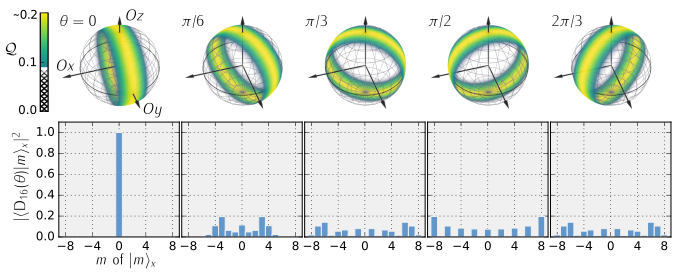
\includegraphics[width=\textwidth]{img/plots/VD_evolution_of_dicke.pdf}
  \caption{Secuence of the evolution of an unpolarized Dicke state of 16 particles for $\Theta=\{i\pi/6\}_{i=0}^4$. Bloch spheres representing the Hirusi distribution of the state, and below PDF of the $J_x$ POVM for each step of the secuence}
\end{figure}

\subsection{Evolution of the expectation values}
Here we show how the expectation values of collective operators needed in this section evolve under the unitary dynamics because of the influence of the homogeneous magnetic field.

\be
  \tr J_x(\Theta) = J_x \text{c}_\Theta - J_y \text{s}_{\Theta}
\ee
